\pdfoutput=1
\documentclass[11pt]{article}
\usepackage{eurosym}
\usepackage[final]{acl}
\usepackage{times}
\usepackage{latexsym}
\usepackage[T1]{fontenc}
\usepackage{graphicx}
\usepackage[utf8]{inputenc}
\usepackage{microtype}
\usepackage{multirow}




\title{University of Bucharest Team at Semeval-2022 Task4: Detection and
	Classification of Patronizing and Condescending Language}

\author{Raluca Andreea G\^inga, {\bf Bogdan Dobre},  \\  {\bf Tudor-Andrei Dumitra\c{s}cu} \and {\bf Bogdan Radu Silviu Sielecki}\\
    University of Bucharest \\
\texttt{\{gingaraluca, dobrebogdan98, }\\
\texttt{tudorandrei.dumitrascu, sieleckiradu\}@gmail.com }
}


\begin{document}
\maketitle

\begin{abstract}
	This report is part of the SemEval 2022 Workshop, Task 4 - Patronizing and
	Condescending Language Detection, trying to find out Patronizing and
	Condescendending Language in any form of text. There were used many methods,
	varying from simple Machine Learning algorithms applied on bag of words
	embeddings until Bert Embeddings and using Neural Networks in order to solve
	both the binary classification and multi-label classification as well.
\end{abstract}

\section{Introduction}

The Patronizing and Condescending Language Detection Task \cite{perezalmendros2022semeval} is based on the
paper Don't Patronize Me! An annotated Dataset with Patronizing and
Condescending Language Towards Vulnerable Communities \cite{perezalmendros2020dont}.

The aim of this task is to identify PCL, and to categorize the linguistic
techniques used to express it, specifically when referring to communities
identified as being vulnerable to unfair treatment in the media.

Participants were provided with sentences in context (paragraphs), extracted
from news articles, in which one or several predefined vulnerable
communities are mentioned. The challenge is divided into two subtasks.

\begin{enumerate}
	\item Subtask 1: Binary classification. Given a paragraph, a system must
	      predict whether or not it contains any form of PCL.

	\item Subtask 2: Given a paragraph, a system must identify which PCL
	      categories express the condescension. The PCL taxonomy has been defined
	      based on previous works on PCL (i.g. Unbalanced power relations, Shallow
          solution, Presupposition, Authority voice, Metaphor, Compassion, The poorer,
          the merrier. )
\end{enumerate}


\section{Background}

The dataset used for this SemEval 2022 task was Don't Patronize Me! dataset,
which contains a suite of sentences that mention some vulnerable communities
and published in media in a lot of English speaking countries. The
paragraphs were manually annotated to show 1) whether the text contains any
kind of PCL, and 2) if it contains PCL, what linguistic techniques
(categories) are used to express the condescension.

The dataset for subtask 1 (binary classification) contained a number of
10.636 paragraphs and 2.792 instances were used for the categories
classification subtask.

In Figure \ref{fig1}, it can be seen that for the first subtask, there are almost
1000 of texts that contain PCL. That means we're dealing with imbalanced
data that we need to solve it. In the next 3 figures (\ref{fig2}, \ref{fig3}
, \ref{fig4}), it could be noticed the distribution of the most common words
both in the full dataset, but in texts that contain/don't contain PCL as
well.

\begin{figure}[ht]
	\centering
	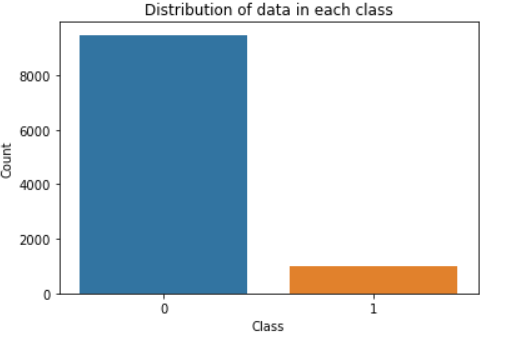
\includegraphics[width=0.4\textwidth]{DataDistribution.png}
	\caption{Classes Distribution for Binary Classification problem (Subtask 1)}
	\label{fig1}
\end{figure}

\begin{figure}[ht]
	\centering
	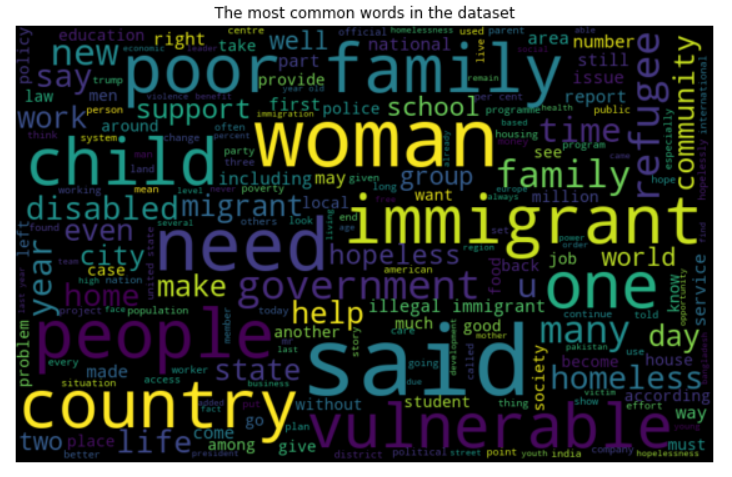
\includegraphics[width=0.4\textwidth]{common.png}
	\caption{Most common words in the dataset (Subtask 1)}
	\label{fig2}
\end{figure}

\begin{figure}[ht]
	\centering
	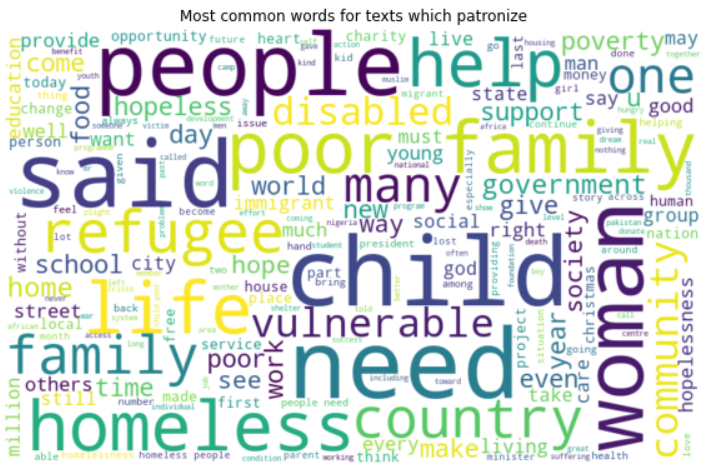
\includegraphics[width=0.4\textwidth]{pcl.png}
	\caption{Most common words classified into PCL}
	\label{fig3}
\end{figure}

\begin{figure}[ht]
	\centering
	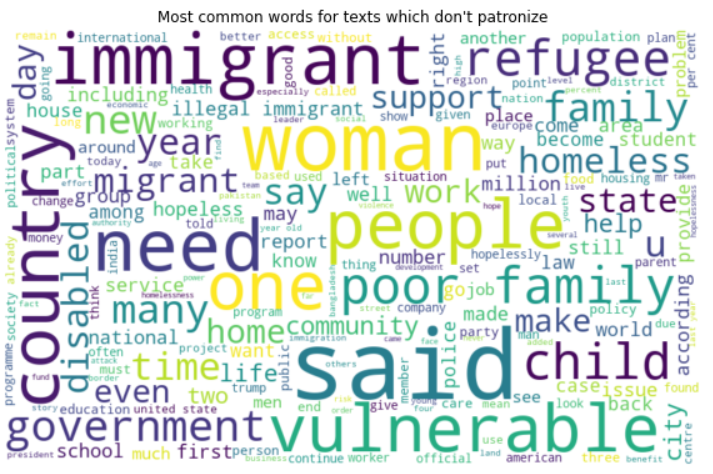
\includegraphics[width=0.4\textwidth]{nopcl.png}
	\caption{Most common words of texts that are not PCL}
	\label{fig4}
\end{figure}


For taks 2, the paragraphs from task 1 are split according to the type of PCL speech category into sentences, resulting in 950 samples.

\section{System Overview}

\begin{enumerate}

	\item Subtask 1 (Binary Classification)

	      Because the dataset was very imbalanced, we tried different approaches in
	      order to make it balanced:

	      \begin{itemize}
		      \item Adding a class weight to the models used. In this approach, we
		            computed a metric in which we obtained a class weight according to the
		            imbalance of the dataset. Through this method, we gave some different
		            weights to both the majority and minority classes. This whole process had
		            the purpose to penalize the misclassification made by the minority class by
		            setting a higher class weight and at the same time, reducing the weight for
		            the majority class.

		      \item Using oversampling methods and special ensemble techniques. In this
		            approach, there were used methods like SMOTE (Synthetic Minority
		            Over-sampling Technique), Adasyn (Adaptive Synthetic), SVM-SMOTE and self
		            paced ensemble that performs strictly balanced under-sampling in each
		            iteration, being very efficient computationally.

		      \item Augmenting the data. Because we notice so little data for label 1, we
		            decided to collect hate speech datasets and add the positive texts into our
		            dataset in order to balance the classes frequency, obtaining a total of 6372
		            from 795 initial texts with label 1. We'll notice in the results section
		            that this collection and generation of new dataset didn't provide good
		            results.
	      \end{itemize}

	      The dataset was a little bit preprocessed and split into two preprocessed
	      types: lemmatized cleaned dataset and stemmed cleaned dataset. These two
	      datasets were generated in order to make some comparison between those two
	      techniques and to see which provided the best results.

	      As feature extraction techniques, there were used techniques like Bag of
	      Words, Tokenizer, Word2Vec and, finally, BertTokenizer which provided the
	      best results in the end.

	      As models, there were used Neural Networks with 3 dense layers, Long Short
	      Term Memory (LSTM) with 64 and 128 neurons with dropout as well, basic
	      Machine Learning algorithms like Logistic Regression, Random Forest, Support
	      Vector Machines as XGBoost. In the end, we decided to try BERT embeddings
	      and a classification BERT model, BertForSequenceClassification, that
	      contains a single linear classification layer on top and that provided the
	      best results after all of the other approaches.

	      Another approach, called "Text shards" made use of the subtask related to
	      multiclass classification as well. For an average text that contains PCL,
	      only some small pieces of them are actually PCL and the rest of the text are
	      not. The assumption is that this confuses the model, because a a combination
	      of pcl and non pcl is labeled as PCL. To address this, the following
	      approach is used:

	      \begin{itemize}
		      \item negative examples are left as they are

		      \item each positive example is replaced with the actual pieces of PCL inside
		            it that we can get from the categories file

		      \item the positive examples obtained this way are added with the negative
		            examples to obtain a training dataset

		      \item all the sentences are cleaned of characters that are not letters and
		            the words in each sentence are lemmatized

		      \item a Tensorflow Hub pretrained model called Universal Sentence Encoder is
		            trained on it

		      \item for each text that we want to predict, we first use the model on the
		            whole text to get an initial label

		      \item a window (of the size of the average length of a cleaned PCL fragment
		            * 2) is slided through the text and the model is used to predict that
		            particular substring. If it is labeled as PCL, then we consider the whole
		            text as PCL.
	      \end{itemize}

	\item Subtask 2 (Multi-label Classification)

	      Considering the fact that the vocabulary of the is English is large,
	      we have tried to leverage the power of pretrained language models.
	      Therefore we have chosen 3 bert-based models which were pretrained
	      for hate speech detection and sentiment analysis. The BERT models
	      also provided a tokenizer which split the sentences into tokens and
	      appended the required tokens.

	      \begin{itemize}
		      \item BERT \cite{bert} Uncased

		      \item  BERT Multilingual Uncased

		      \item BERT HateXplain \cite{mathew2020hatexplain}: This model was trained to classify text as Hate speech, Offensive or Normal.
		            It was trained on Gab, Twitter and Humain Rationale;

		      \item Distil BERT : This model is a version of Distilled bert finetuned on the Twitter dataset;

		      \item Distil BERT Multilingual Cased \cite{DistilBERT}

		      \item Distill RoBERTa : This model is a verion of Distilled RoBERTa finetuned on the Twitter dataset;
	      \end{itemize}

	      In the paper describing the dataset \cite{perezalmendros2020dont},
	      the authors group the categories into 3 General categories.

	      \begin{enumerate}
		      \item The saviour: Unbalanced power relations and Shallow relations

		      \item  The Expert: Presupposition and Authority voice

		      \item The Poet: Compassion, Metaphor and The poorer the merrier

	      \end{enumerate}

	      From this idea, we tried to train the models to predict those 3
	      categories, and save the hidden features to a fixed latent space.
	      Then these learned features can be used when training the model to
	      predict the required 7 sub-classes.

	      Along with those bert-based model, we also tried to implement models based on Word2Vec\cite{goldberg2014word2vec}
	      trained on "Google News" and Machine Learning algorithms based on TF-IDF and BOW:

	      \begin{itemize}
		      \item LSTM Word2Vec Embeddings \cite{staudemeyer2019understanding}
		      \item biLSTM Word2Vec Embeddings \cite{huang2015bidirectional}
		      \item RNN Word2Vec Embeddings \cite{rnn}
		      \item SVM TF-IDF
		      \item RandomForest TF-IDF
	      \end{itemize}



	      We also dabbled with the thought of training our own Word2Vec, in
	      order to create a model specialized on hate speech. However we
	      decided against this idea, due to the lack of usable datasets and the
	      computational resources required for this task.


\end{enumerate}


\section{Results}

\begin{enumerate}
	\item Subtask 1 (Binary Classification)

	      \begin{enumerate}
		      \item Deep Learning / Machine Learning for Imbalanced and Oversampled
		            dataset

		            \scalebox{0.5}{
			            \begin{tabular}[t]{|l|l|l|l|l|l|l|l|l|}
				            \hline
				                                    & \multicolumn{4}{|c|}{Lemmatized (F1\_Score)}                            \\ \hline
				            Approach                & Simple                                       & SPE  & SMOTE  & SVMSMOTE
				            \\ \hline
				            Neural Networks         & 0.27                                         & -    & 0.2823 & 0.3187
				            \\ \hline
				            Logistic Regression     & 0.34                                         & -    & 0.35   & 0.35     \\
				            \hline
				            Random Forest           & 0.067                                        & 0.31 & 0.19   & 0.16     \\
				            \hline
				            Support Vector Machines & 0.27                                         & -    & 0.10   & 0.14     \\
				            \hline
				            XGBoost                 & 0.15                                         & -    & 0.23   & 0.24     \\ \hline
			            \end{tabular}
		            }

		            \scalebox{0.5}{
			            \begin{tabular}[t]{|l|l|l|l|l|l|l|l|l|}
				            \hline
				                                    & \multicolumn{4}{|c|}{Stemmed (F1\_Score)}                           \\ \hline
				            Approach                & Simple                                    & SPE  & SMOTE & SVMSMOTE
				            \\ \hline
				            Neural Networks         & 0.2698                                    & -    & 0.289 & 0.3166
				            \\ \hline
				            Logistic Regression     & 0.35                                      & -    & 0.38  & 0.37     \\
				            \hline
				            Random Forest           & 0.038                                     & 0.31 & 0.21  & 0.13     \\
				            \hline
				            Support Vector Machines & 0.27                                      & -    & 0.14  & 0.20     \\
				            \hline
				            XGBoost                 & 0.17                                      & -    & 0.23  & 0.24     \\ \hline
			            \end{tabular}
		            }

		      \item Tokenization of the lemmatized and stemmed dataset / Word2Vec + LSTM
		            neural network

		            \scalebox{0.5}{
			            \begin{tabular}[t]{|l|l|l|l|l|}
				            \hline
				                               & \multicolumn{2}{|l}{Lemmatized (F1\_Score)} & \multicolumn{2}{|l|}{Stemmed
				            (F1\_Score)}                                                                                                        \\ \hline
				            Approach           & Simple                                      & Word2Vec                     & Simple & Word2Vec \\ \hline
				            LSTM (64 neurons)  & 0.2693                                      & 0.2109                       & 0.3213 & 0.2093   \\ \hline
				            LSTM (128 neurons) & 0.2317                                      & 0.2308                       & 0.2789 & 0.2412   \\ \hline
			            \end{tabular}
		            }

		      \item Data augmentation

		            \scalebox{0.5}{
			            \begin{tabular}[t]{|l|l|}
				            \hline
				                                    & Augmented Data (F1\_Score) \\ \hline
				            NNs with 3 layers       & 0.2155                     \\ \hline
				            Logistic Regression     & 0.23                       \\ \hline
				            U.S.E. + 2 dense layers & 0.2316                     \\ \hline
			            \end{tabular}
		            }

		      \item BERT Transformers + BertForSequenceClassification

		            \scalebox{0.55}{
			            \begin{tabular}[t]{|l|l|}
				            \hline
				                                        & Unprocessed data (F1\_Score) \\ \hline
				            Bert Tokenizer + Classifier & 0.5074                       \\ \hline
			            \end{tabular}
		            }

		      \item Text shards

		            \scalebox{0.55}{
			            \begin{tabular}[t]{|l|l|}
				            \hline
				                                        & Lemmas F1\_Score \\
                                                        & \\ \hline
				            Text shards & 0.3117                       \\ \hline
			            \end{tabular}
		            }
	      \end{enumerate}

	\item Subtask 2 (Multiclass Classification)

	      \begin{enumerate}
		      \item Bert models approach for classification across 7 classes. In the table it
                      can be seen that the models can easily two of the categories,
                      while the rest of them are not learned

		            \scalebox{0.7}{
			            \begin{tabular}[t]{|l|l|l|l|l|l|l|l|l|}
				            \hline
				                          & \multicolumn{4}{|c|}{F1 Score}                            \\ \hline
				            Class      & Unb& Sha  & Pre  & Aut
				            \\ \hline
				            Bert          & 0.82 & 0.0 & 0.0 & 0.0
				            \\ \hline
				            DistilRoberta & 0.83 & 0.0 & 0.0 & 0.0   \\
				            \hline
				            Distilbert    & 0.82 & 0.0 & 0.0 & 0.0   \\
                            \hline
			            \end{tabular}
		            }
		            \scalebox{0.7}{
			            \begin{tabular}[t]{|l|l|l|l|l|l|l|l|l|}
				            \hline
				                          & \multicolumn{4}{|c|}{F1 Score}                            \\ \hline
                            Class      & Met & Com  & Mer  & Mean Score
				            \\ \hline
                            Bert          & 0.0  & 0.0  & 0.64 & 0.21
				            \\ \hline
                            DistilRoberta & 0.0  & 0.0  & 0.59 & 0.20    \\
				            \hline
                            Distilbert    & 0.66 & 0.08 & 0.0  & 0.34   \\
                            \hline
			            \end{tabular}
		            }
                \item The general class aproach is detailed in the following tables.
                    It shows that the general classes were learned, but when using the
                    pretrained models and fine-tuning on the specific classes, some
                    of previously learned features are lost.

                        \scalebox{0.8}{
                            \begin{tabular}[t]{|l|l|l|l|l|l|l|l|l|}
                                \hline
                                 & \multicolumn{3}{|c|}{F1 Score}\\
                                \hline
                                Main/Sub-classes& Expert & Aut  & Pre \\
                                \hline
                                Bert          & 0.44  & 0.0  & 0.0 \\
                                \hline
                                DistilRoberta & 0.54  & 0.0  & 0.0 \\
                                \hline
                                DistilBert    & 0.42 & 0.0 & 0.40  \\
                                \hline
                                DistilBertMLC & 0.36 & 0.0 & 0.0  \\
                                \hline
                            \end{tabular}
                        }

                        \scalebox{0.7}{
                            \begin{tabular}[t]{|l|l|l|l|l|l|l|l|l|}
                                \hline
                                 & \multicolumn{3}{|c|}{F1 Score}\\
                                \hline
                                Main/Sub-classes& Saviour & Sha  & Unb \\
                                \hline
                                Bert          & 0.85 & 0.0 & 0.84 \\
                                \hline
                                DistilRoberta & 0.85 & 0.0 & 0.84 \\
                                \hline
                                DistilBert    & 0.75 & 0.0 & 0.81  \\
                                \hline
                                DistilBertMLC & 0.86 & 0.0 & 0.83  \\
                                \hline
                            \end{tabular}
                        }

                        \scalebox{0.7}{
                            \begin{tabular}[t]{|l|l|l|l|l|l|l|l|l|}
                                \hline
                                 & \multicolumn{4}{|c|}{F1 Score}\\
                                \hline
                                Main/Sub-classes& Poet & Com  & Mer & Met \\
                                \hline
                                Bert          & 0.69 & 0.0 & 0.0 & 0.59 \\
                                \hline
                                DistilRoberta & 0.69 & 0.11 & 0.0 & 0.65 \\
                                \hline
                                DistilBert    & 0.61 & 0.0 & 0.0 & 0.67  \\
                                \hline
                                DistilBertMLC & 0.60 & 0.0 & 0.0 & 0.52  \\
                                \hline
                            \end{tabular}
                        }
	      \end{enumerate}
\end{enumerate}


\section{Conclusion}

In the current project, it was solved the problem posed by SemEval 2022 Task
4: Patronizing and Condescending Language Detection. There were applied
various methods, including the application of Word Embeddings (Bag of Words,
Word2Vec, BERT), tokenization, oversampling/undersampling of the datasets.

In the binary classification problem, the approach that gave the best result
on the validation dataset was BERT transformers combined with Bert for
Sequence Classification, obtaining 0.50 as f1\_score.

In the multi classification multi label task, the number of labels proved to
be a challenge. The results overall are low and the models are only able to learn
only a few classes. The general class approach also proved to be inneficient.

Some recommendations for future work could be to have a better approach and introduce
more linguistic insignt in the approach.

\section*{Acknowledgements}

We would like to thank our supervisor Ana-Sabina Uban for the guidance and throughout
the development of the project.



\bibliography{custom}
\end{document}

